\documentclass[a4paper,12pt]{article}
\usepackage[utf8]{inputenc}
\usepackage[T1]{fontenc}
\usepackage[hungarian]{babel}
\usepackage{graphicx}
\usepackage{geometry}
\geometry{a4paper,
		     tmargin = 35mm, 
		     lmargin = 25mm,
		     rmargin = 30mm,
		     bmargin = 30mm}
\usepackage{mathtools}
\usepackage{amsmath}
\usepackage{color}
\usepackage{setspace}
\usepackage{amsmath,amssymb}
\usepackage{float}
\usepackage{hyperref}

\usepackage{indentfirst}
\usepackage{subfig}

\usepackage{siunitx}

\renewcommand\thesection{\Roman{section}}

\begin{document}

\linespread{1.25}

\begin{titlepage}

	\centering
	
\includegraphics[width=0.66\textwidth]{elte.jpg}\par\vspace{1cm}
	{\scshape\LARGE ELTE TTK \par}
	\vspace{3cm}
	{\scshape\Large Röntgendiffrakció \par}
	\vspace{1cm}
	{\large\itshape Olar Alex\par}
	\vspace{3cm}
	{\large 2018 \par}
	
\end{titlepage}

\tableofcontents

\newpage

\section{Elméleti összefoglaló, mérési eszközök}

\par A mérés során 4 feladatot végeztünk el. Ennek során egy vas-alumínium ötvözetet vizsgáltunk először, melynek a rácsszerkezetét kellett meghatároznunk, majd egy alumínium-magnézium ötvözetre tértünk át, amiben a magnézium arányát kellett meghatároznunk megváltozott rácstávolság alapján. Majd egy ismeretlen minta (szén-pasztilla) csúcskiszélesedése alapján meg lehetett határozni az ismeretlen fázist. Végül egy otthoni feladatot kaptunk a rácsparaméter otthoni meghatározására.

\section{Kiértékelés}

\subsection{Rácstípus maghatározása $Fe-Al$ ötvözet}

\par A reflexiók indexelésével meghatároztuk a difraktorgramból, hogy az ötvözet $BCC$ rács. Ezt a következőképpen kiviteleztük:

\begin{itemize}
\item meghatároztuk a Bragg-egyenlet alapján, ($2d_{hkl}sin\vartheta = \lambda$), a $d_{hkl}$ értékeket, majd leosztva az első diffrakciós csúcshoz tartozó $d_{hkl}$ értékkel az egész sort, kaptuk a közelítő $N$ értékeket
\end{itemize} 

\begin{figure}[H]
\centering
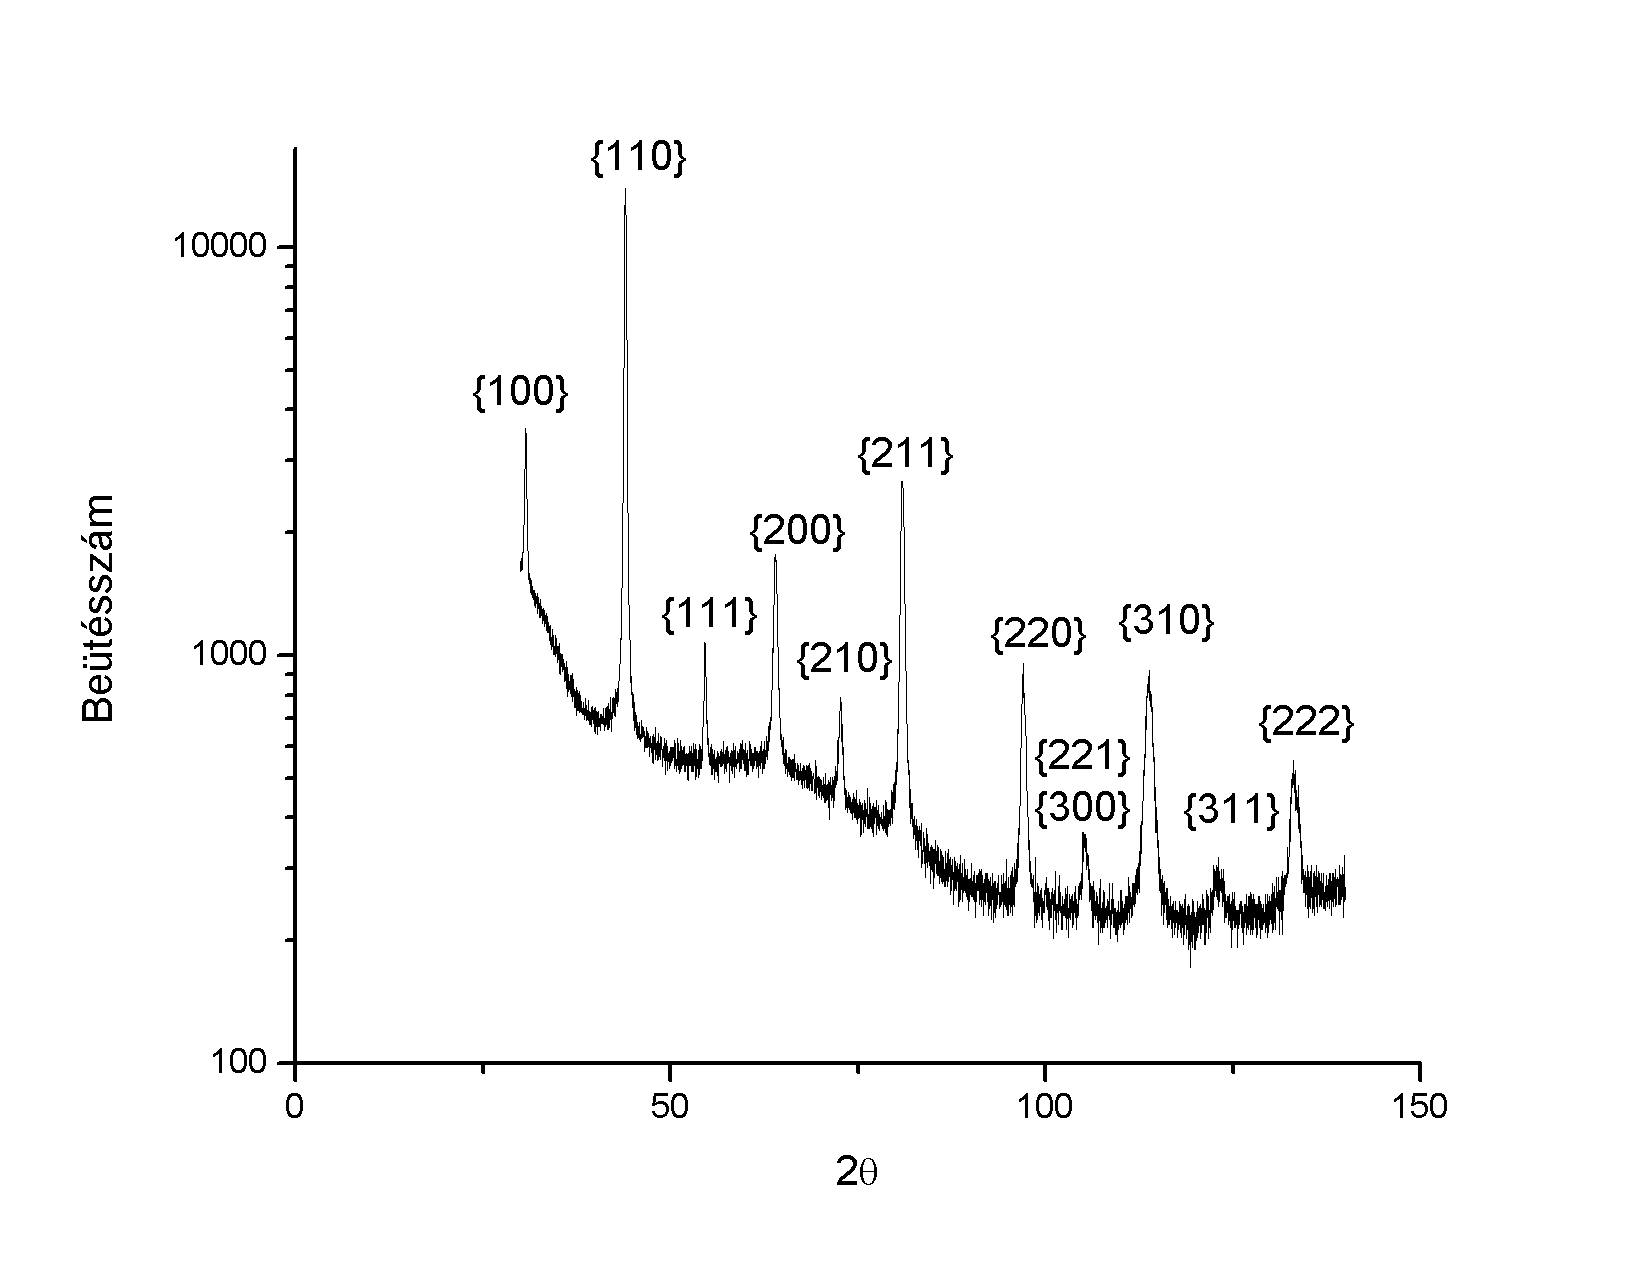
\includegraphics[width=0.8\textwidth]{./fel1.png}
\caption{$Fe-Al$ ötvözet röntgen spektruma}
\end{figure} 

\begin{center}
\begin{tabular}{|c|c|c|}
\hline
$2\vartheta$ & $d_{hkl}$ [$\si{\angstrom}$] & N \\
\hline
30.7 &2.9121 & 1 \\
\hline
44.0 & 2.058 & 2.003 \\
\hline
54.6 & 1.681 & 3.002 \\
\hline
64.0 & 1.455 & 4.007 \\
\hline
72.6 & 1.302 & 5.002 \\
\hline
80.9 & 1.188 & 6.007 \\
\hline
97.1 & 1.029 & 8.017 \\
\hline
105.3 & 0.97 & 9.018 \\
\hline
113.8 & 0.92 & 10.015 \\
\hline
123.0 & 0.877 & 11.022 \\
\hline
133.2 & 0.84 & 12.02 \\
\hline
\end{tabular}
\end{center}

\par Ebből jól látható, hogy jó közelítéssel egész $N$ értékeket kaptunk, amiből látható, hogy ez egy $BCC$ rács, hiszen:

\begin{equation*}
\frac{1}{d_{hkl}^{2}} = \frac{1}{a^{2}}N = \frac{1}{a^{2}}(h^{2} + k^{2} + l^{2})
\end{equation*}

\par összefüggést csak köbös rácsra lehet alkalmazni.

\subsection{Ötvözőkoncentráció meghatározása}

\par Az alumínium magnézium szennyezettségét kellett meghatározni diffrakcióból. A kapott diffrakciós görbén leolvastuk a $2\vartheta$ szögeket, majd kiszámoltuk ebből a $d_{hkl}$ mennyiségeket. Itt a szükséges $N$ értékeket megkaptuk, hiszen a Miller-indexek egy kapott fájlban fel voltak sorolva. A mért és számolt adatokat táblázatba foglalva:

\begin{figure}[H]
\centering
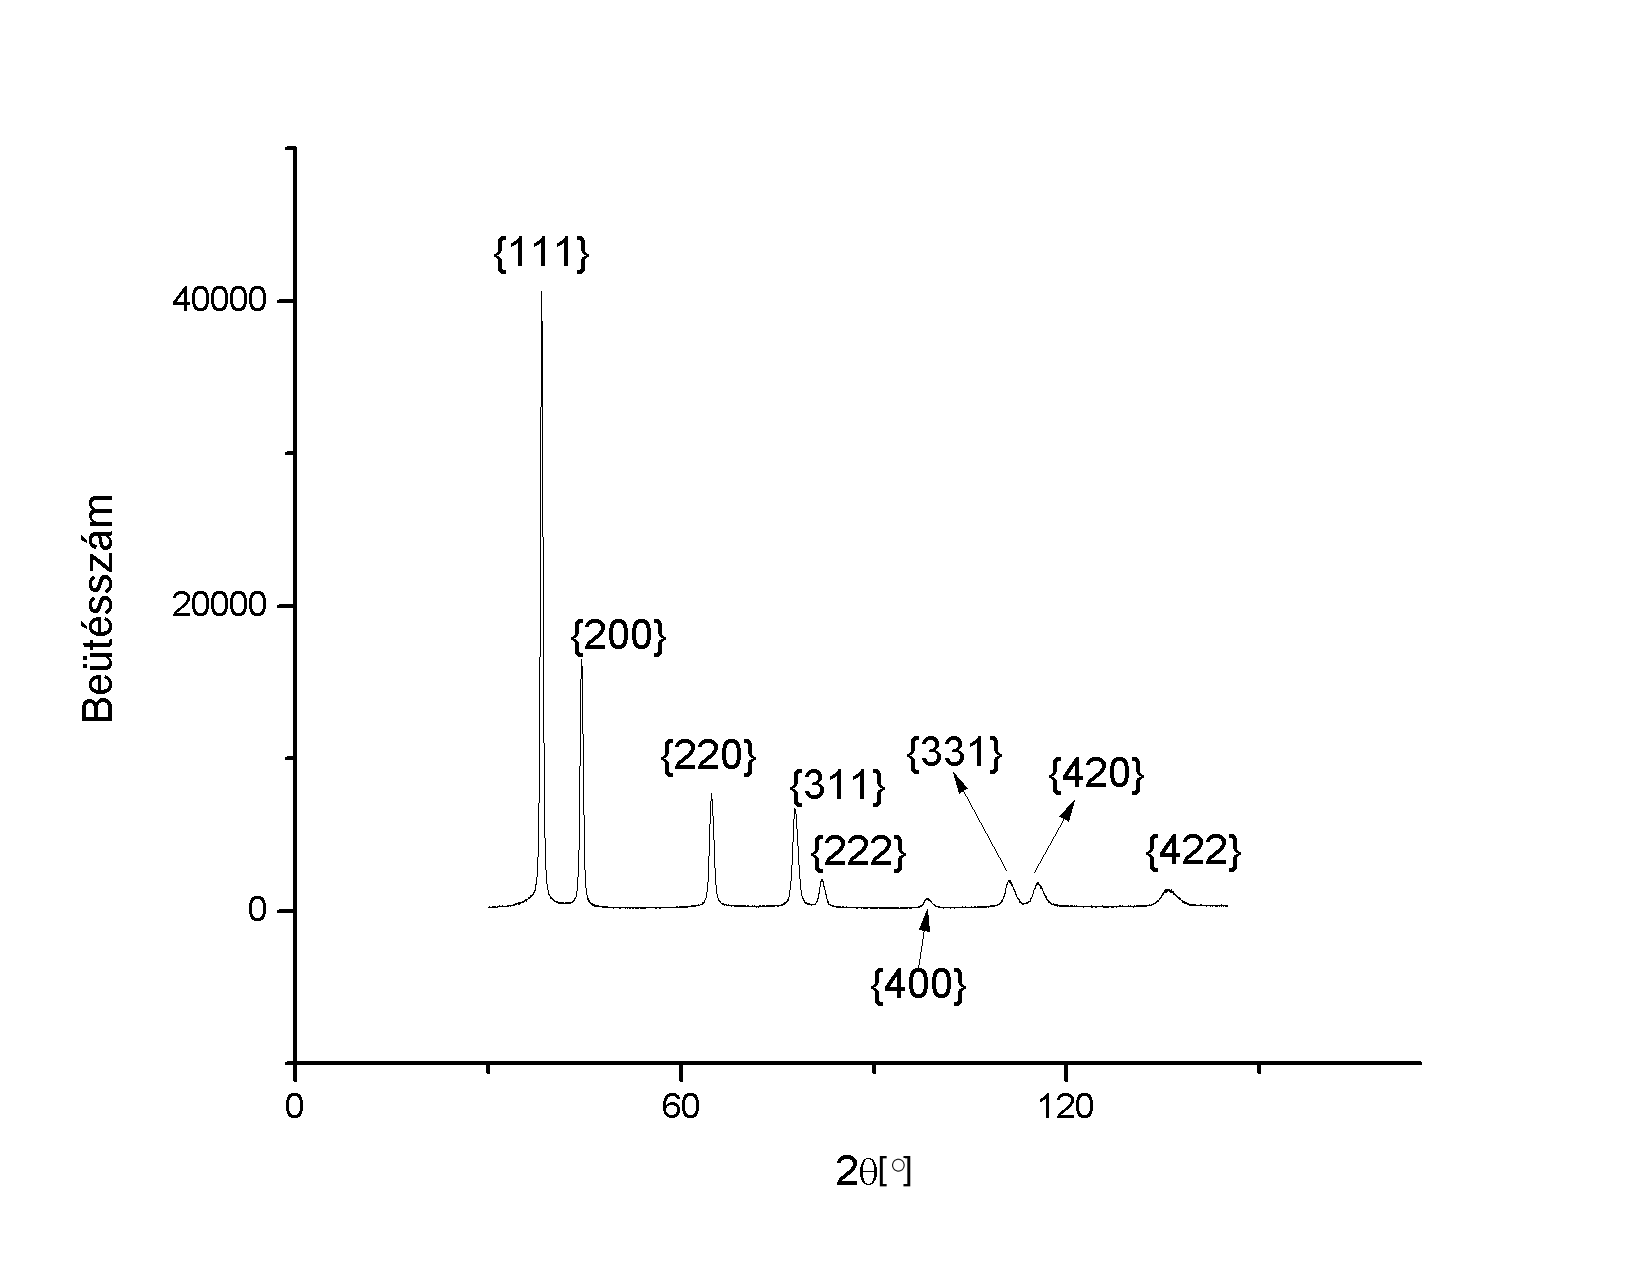
\includegraphics[width=0.7\textwidth]{./fel2.png}
\caption{$Mg$-mal szennyezett $Al$ röntgen spektruma}
\end{figure} 

\begin{center}
\begin{tabular}{|c|c|c|c|}
\hline
$2\vartheta$ & $d_{hkl}$ [$\si{\angstrom}$] & N & $a_{hkl}$ [$\si{\angstrom}$] \\
\hline
38.3 &2.35 & 3 & 4.07\\
\hline
44.52 & 2.035 & 4 & 4.07 \\
\hline
64.75 & 1.44 & 8 & 4.072\\
\hline
77.76 & 1.228 & 11 & 4.073\\
\hline
81.95 & 1.176 & 12 & 4.073 \\
\hline
98.38 & 1.019 & 16 & 4.074\\
\hline
111.15 & 0.935 & 19 & 4.074\\
\hline
115.56 & 0.911 & 20 & 4.075\\
\hline
135.9 & 0.832 & 24 & 4.075\\
\hline
\end{tabular}
\end{center}

\par A szennyezés miatt $a_{hkl}$ változik a következő formula szerint:

\begin{equation*}
a_{hkl} = a_{0} - Dcos\vartheta\Big(ctg\vartheta + \frac{cos\vartheta}{\vartheta}\Big) = a_{0} - D\cdot f(\vartheta)
\end{equation*}

\par ebből jól látható, hogy $a_{hkl} - f(\vartheta)$ változók között lineáris összefüggés van. Erre egyenest illesztve:

\begin{figure}[H]
\centering
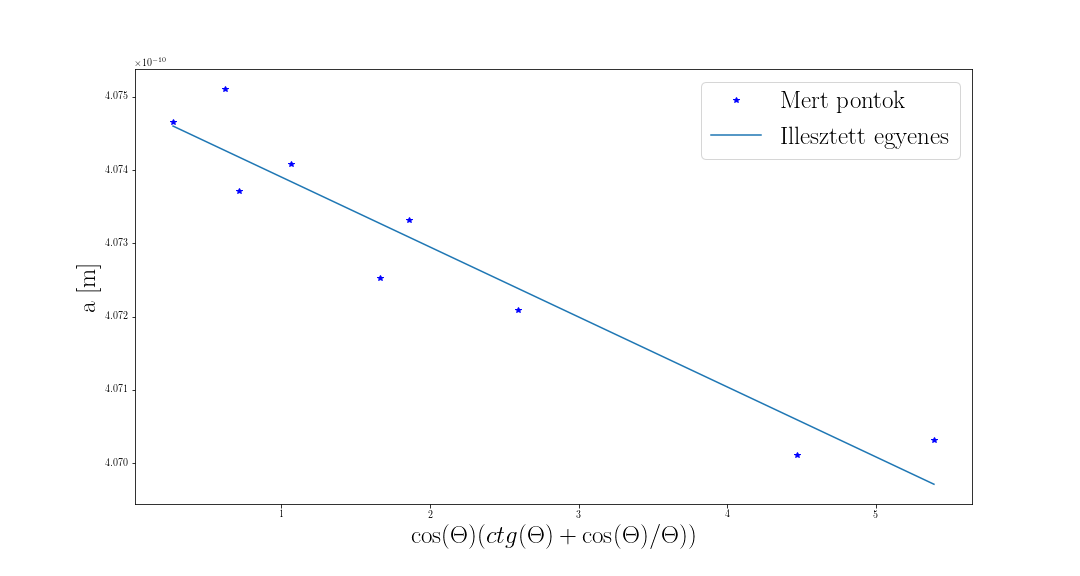
\includegraphics[width=1\textwidth]{./egyenes.png}
\caption{Lineáris összefüggés $a_{hkl}$ és $f(\vartheta)$ között}
\end{figure} 

\par Ahonnan az illesztési paraméterek ($a_{0}$ hibája olyan kicsi lett, hogy felülbecsültem):

\begin{equation*}
D = (9.542 \pm 1.128) \cdot 10^{-14} ~m \quad \quad
a_{0} = (4.075 \pm 0.001) \cdot 10^{-10} ~m
\end{equation*}

\par Nagyban befolyásolja az illesztést, ha a csúcsokat nem kellő értékes jegyre adjuk meg.

\par Ezután le tudtuk olvasni, hogy $a_{0}$-hoz milyen $Mg$ koncentráció tartozik. Ehhez szükségünk van egy ilyen függvényre, ami ezt megmutatja. Ehhez a labor során kaptunk egy adatsort, amiből az derült ki, hogy $(6.0537 \pm 0.001)\%$ részarányban tartalmaz az alumínium minta magnéziumot.

\begin{figure}[H]
\centering
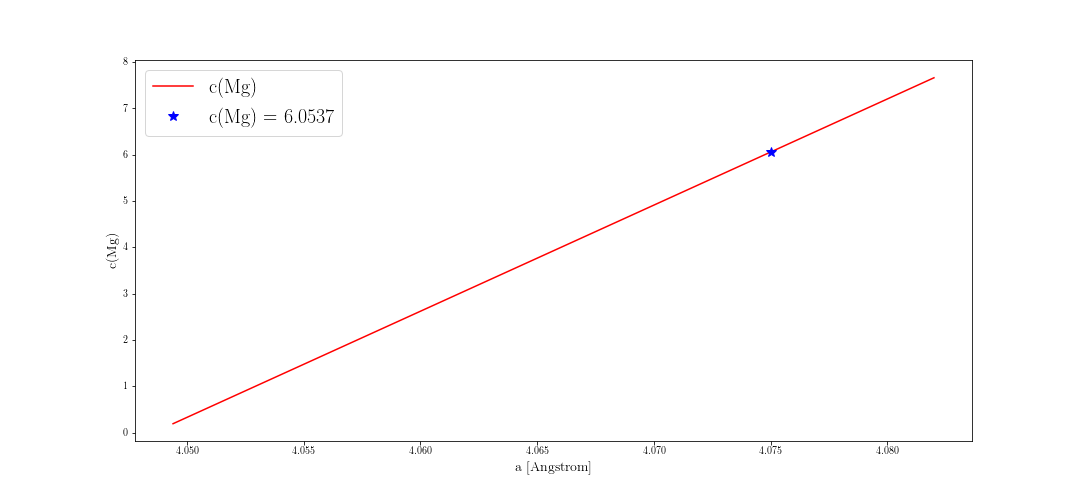
\includegraphics[width=.96\textwidth]{./konc.png}
\caption{Lineáris összefüggés a koncentráció és $a_{hkl}$ között, jelölve a mért pont}
\end{figure} 

\subsection{ Ismeretlen fázis meghatározása}

\par Ismeretlen mintáról felvett röntgendiffrakciós diagramot véve, az első három csúcsra kerestünk az adatbázisban. 

\begin{figure}[H]
\centering
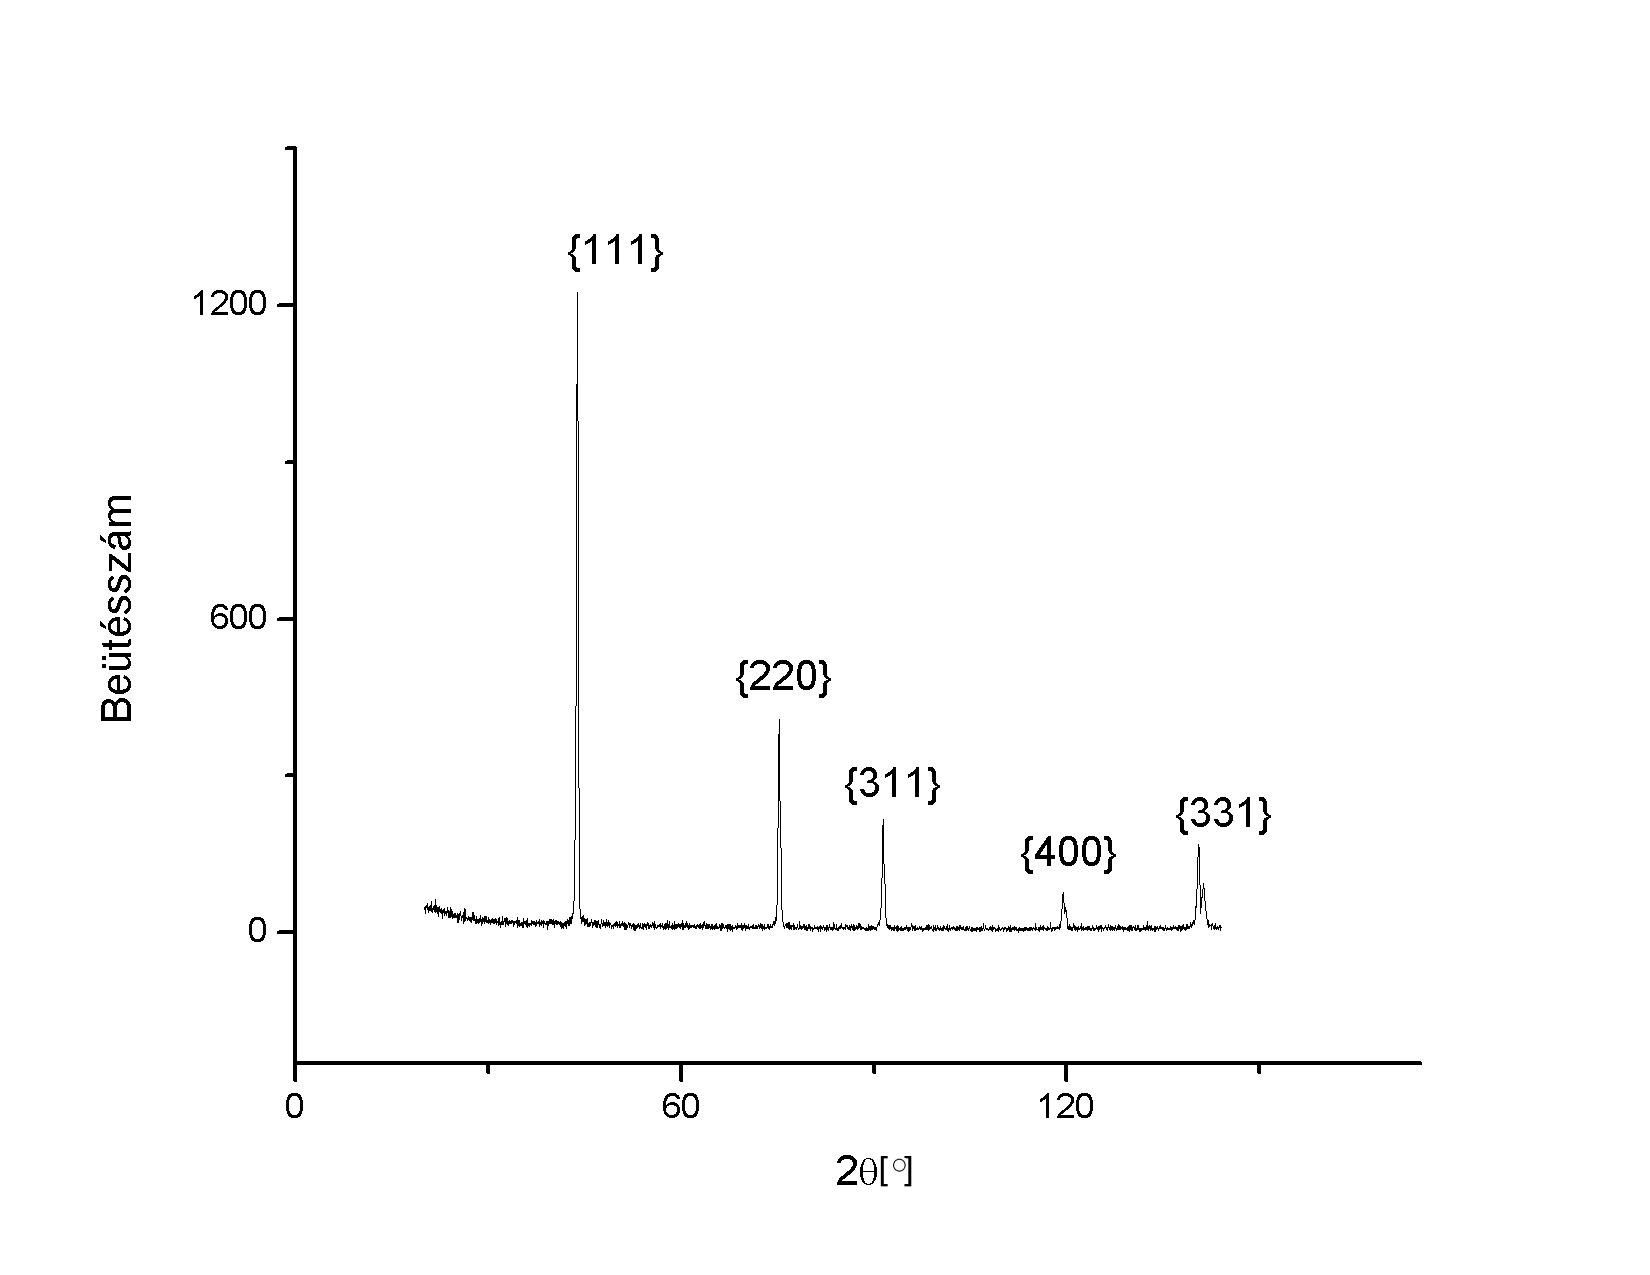
\includegraphics[width=.5\textwidth]{./fel3.png}
\caption{Ismeretlen minta}
\end{figure}

\begin{center}
\begin{tabular}{|c|c|c|}
\hline
$2\vartheta$ & $d_{hkl}$ [$\si{\angstrom}$] \\
\hline
43.846 & 2.065 \\
\hline
75.247 & 1.263  \\
\hline
91.471 & 1.076 \\
\hline
119.564 & 0.892 \\
\hline
140.826 & 0.818\\
\hline
\end{tabular}
\end{center}

\par Az adatbázisból megkaptuk, hogy egy $C$ mintáról van szó. Később megtudtuk, hogy valóban egy szén-pasztillát mértünk.

\begin{figure}[H]
\centering
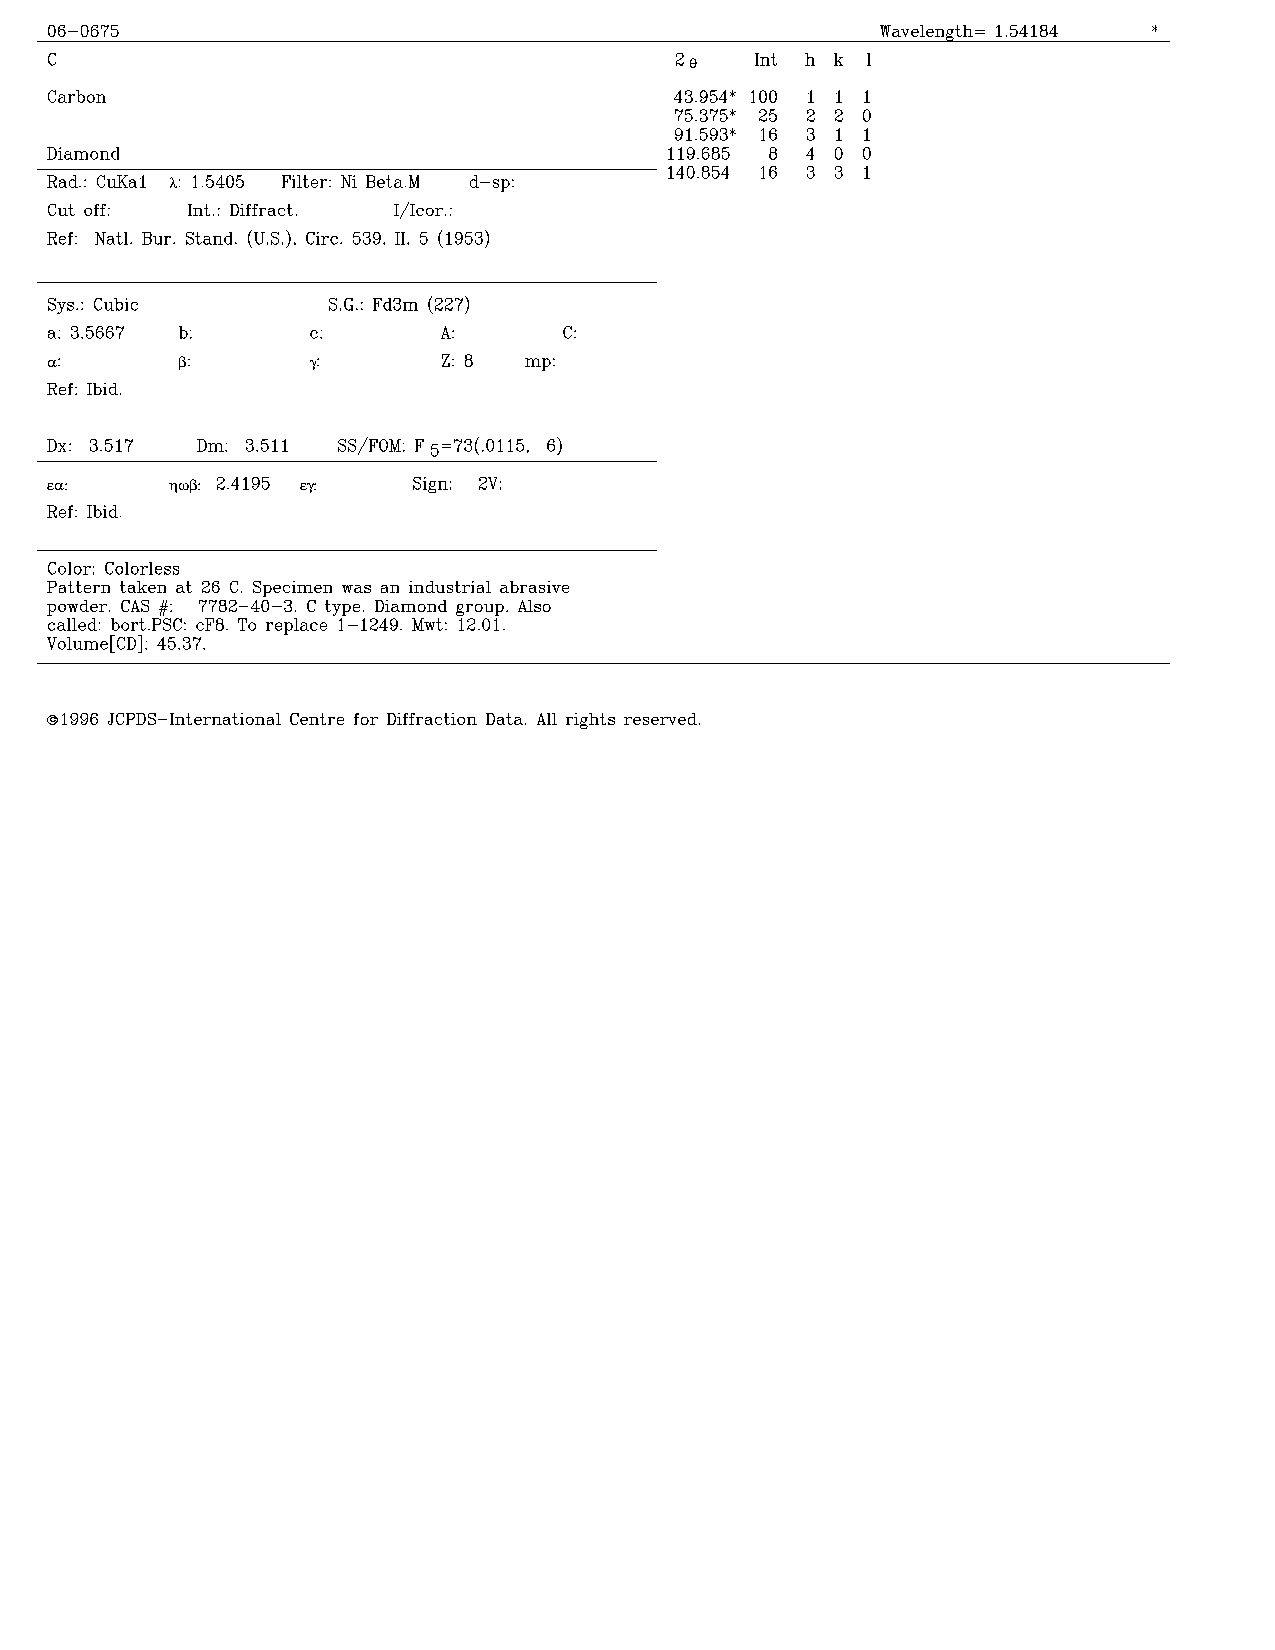
\includegraphics[width=.88\textwidth]{./maad.pdf}
\end{figure}

\subsection{ Si minta rácsparaméterének meghatározása}

\par A kapott adatok alapján 

\begin{center}
\begin{tabular}{|c|c|c|c|}
\hline
$2\vartheta$ & $d_{hkl}$ [$\si{\angstrom}$] & N & $a_{hkl}$ [$\si{\angstrom}$] \\
\hline
38.3 &2.35 & 3 & 4.07\\
\hline
44.52 & 2.035 & 4 & 4.07 \\
\hline
64.75 & 1.44 & 8 & 4.072\\
\hline
77.76 & 1.228 & 11 & 4.073\\
\hline
81.95 & 1.176 & 12 & 4.073 \\
\hline
98.38 & 1.019 & 16 & 4.074\\
\hline
111.15 & 0.935 & 19 & 4.074\\
\hline
115.56 & 0.911 & 20 & 4.075\\
\hline
135.9 & 0.832 & 24 & 4.075\\
\hline
\end{tabular}
\end{center}

\end{document}